\documentclass{sig-alt-release2}
\usepackage{url}
\usepackage{hyperref}
\usepackage{color}
\usepackage{graphics,graphicx}

\usepackage{epsfig}
\usepackage{epstopdf}

\usepackage{colortbl}
\usepackage{multirow}
\usepackage{booktabs}
\usepackage{ifthen}  

\graphicspath{ {./img/} }

\begin{document}
\newcommand{\todo}[1]{\textcolor{red}{#1}}
\def\newblock{\hskip .11em plus .33em minus .07em}

\conferenceinfo{DIM3} {2010, Glasgow, UK} 
\CopyrightYear{2010}
\clubpenalty=10000
\widowpenalty = 10000

\title{{Report Name}}

\numberofauthors{1}
\author{
\alignauthor
Author Names\\
	   \affaddr{Group Name}\\
      \affaddr{itech/Dim3}\\
      \affaddr{Student no.s}\\
             \email{\{ name1, name2, name3, name4\}@students.glasgow.ac.uk }
}
\maketitle

\begin{abstract}
Provide a concise summary of the design of the application

\end{abstract}

\section{Aim of Application}

%\item	What is the purpose of the application?
%\item	Eg. The application is an academic search engine called AcaSe and is it is based upon the PuppyIR Framework\cite{glassey2011framework}, which has been used to construct other such services\cite{glassey2010fifi,elliot2010fifi}. The main purpose of this web application is to provide a customized interface to services such as Google Scholar and MS Academic Search. 
%\item	What are the assumptions about the aims and objectives?
%\item	Describe the design goals and objectives of the application.
%\item	What are the constraints of the project?
%\item	Functionality List: i.e. what is the required and desired functionality?
%\item	Reflective Questions: 
%\item	Is the scope of the application appropriate? 
%\item	Are the design goals realistic/achievable? 
%\item	How complex is the application? 
%\item	Is distribution across the web appropriate?

This application is a media playlist creator and viewer allowing users to share their playlists with others and view the playlists of other users. The main purpose of the application is to allow users to create media playlists and view both their own playlists and playlists created by other users.

At the start of the project we had the following main goals:
\begin{itemize}
\item To create a simple and intuitive interface which allowed users to create playlists easily and quickly with minimal switching between different pages during the process of adding media.
\item To allow users to create playlists including media from a number of different sources.
\end{itemize}

The following list contains the required functionality for the application:

\begin{itemize}
\item Register/Login
\item Create Playlists
\item Add Media to Playlists
\item View Media in Playlists
\end{itemize} 

\section{Client Interface}
\begin{itemize}
\item	Draw a wireframe of the user interface
\item	this may require several wireframes depending on the complexity of the application and the interfaces
\item	Describe the user interface.
\item	i.e. Label key input and output components: describe them.
\item	Provide a Walkthrough and explain the user interactions with application. 
\item	i.e. use cases
\item	Describe the interactions associated with the dynamic components on the user interface.
\item	What calls are required to dynamically update the data on the client side?
\item	How does the user interface help the user achieve their goal, or complete their task? 
\item	Is the user interface intuitive, appealing, usable, etc?
\item	What technologies are used on the client side? 
\item	What are the reasons for your choices? i.e. what is the advantages and disadvantages of using this technology? 
\item	What other options are there? 
\end{itemize}

\section{Application Architecture}
\begin{itemize}
\item	N-Teir Architecture Diagram
\item	i.e. data flow diagram between the interface/client, middle ware, and backend services/data repos
\item	Describe the data model i.e. what data needs to be stored or persisted by the application?
\item	What are the relationships within the data model.
\item	i.e. use ER diagram and explain.
\item	Describe the backend services used (if any).
\item	Reflective Questions: 
\item	How have you ensured that there is a separation of concerns? 
\item	What other technology could have been used instead of django? 
\item	What are the advantages of using a Web Application Framework over other technology? 
\item	And, what are the disadvantages?
\end{itemize}

\begin{figure}[h]
  \begin{center}
    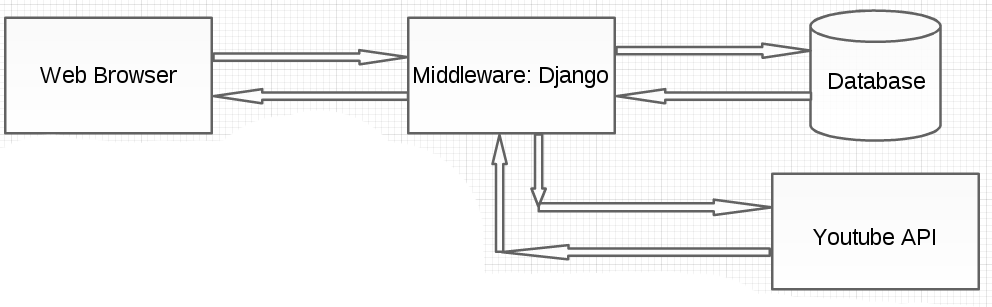
\includegraphics[width=0.45\textwidth]{ntier}
    \caption{N-Tier Diagram} \label{fig:n-tier}
  \end{center}
\end{figure}

\begin{figure}[h]
  \begin{center}
    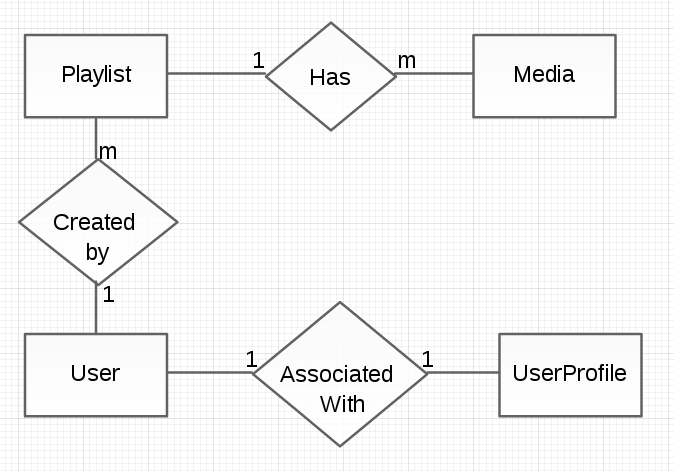
\includegraphics[width=0.45\textwidth]{ER}
    \caption{Entity-Relationship Diagram} \label{fig:ER}
  \end{center}
\end{figure}




\section{Message Parsing}
\begin{itemize}

\item	On the architecture diagram, Identify and label the main messages that will be parsed through the application.
\item	or alternatively (and preferably) include sequence diagrams to denote the sequence of communications parse between clients and servers.
\item	Describe the messages that are parsed back and forth through the application.
\item	For the main transactions - describe the payload of the messages 
\item	i.e. What are the contents of the messages? i.e. include sample XML, XHTML, JSON, etc of one or two messages.
\item	What is the format of the messages? 
\item	Why this format? 
\item	What other formats could be used, what are the advantages and disadvantages of these other formats?
\end{itemize}

%%%%%%%%%%%%%%%%%%%%%%%%%%%%%%%%%%%%%%%%%%%%%%%%%%%%%%%%%%%%%%%%%%%%%%%%

\section{Implementation Notes}

\subsection{Views}
%\item Views - What are the main views that you have implemented and what do they do?

The main views we created for the project were as follows:

\begin{itemize}
\item Index - This view loads the index.html template and populates it with data for the current user. It gets a list of all of the playlists and then gets a seperate list of playlists which created by the current user. This view also deals with registering users and logging users in by saving the data entered into the relevant form on the index page.
\item Playlist - The playlist view deals with the add\verb=_=media function by verifying the form passed to the function is valid, extracting the data from the form and then performing the appropriate function calls to add the media to the database. This view also populates the context dictionary with the correct media when the playlist page is opened.
\end{itemize}

\subsection{URL Mapping Schema}
%\item URL Mapping Schema - what is your URL mapping and schema?

The URL mapping schema we decided to use was designed to be fairly easy to read and aquire information from. Every URL begins with the IP then `/allthemedia/'. The next section contains information about the type of page the user is accessing, for example `/login/', `/register/', `/about/', `/user/' etc. If this section contains `/user/' then the user is accessing a page with information relating to a specific user. This is followed by `/user/[username]/' to view the user profile of a particular user. This can be followed by a playlist title to view a playlist created by the specified user i.e. `/allthemedia/user/joe/coolsongs/' would display the playlist called `coolsongs' which was created by the user called `joe'. Anything beyond this stage specifies actions to be performed on a particular playlist, such as add\verb=_=media.

\subsection{External Services}
%\item External Services  - what external services does your application include and what handlers did you include?

The main external service used by our application is YouTube. This is used extensively by our 'Playlist' page, the main feature of which is a large YouTube player which plays the playlist media. This is created using the YouTube API which then displays the media from the current playlist.

\subsection{Functionality}
%\item	Functionality Checklist (which functionality is completed)

The folowing functionality is completed:

\begin{itemize}
\item Login/Logout/Register
\item Create playlists
\item View playlists
\item Adding media to a playlist from the 'add\verb=_=media' page
\item Auto-playing videos in a playlist
\item Skipping forwards and backwards through a playlist
\end{itemize}

%\item	Known Issues (what kind of works, what kind of errors to do you get)

The following functionality is unfinished, buggy or unimplemented:

\begin{itemize}
\item Adding to a playlist from the form on the playlist page - currently re-loads the playlist page with no playlist loaded and without adding the new media.
\item CSS missing from add\verb=_=media page - we had intended to add media from the playlist page and the add\verb=_=media was supposed to be a temporary page. However, because this feature remains unfinished, the add\verb=_=media page is the only way to add media to a playlist.
\item After adding media to a playlist the re-direct goes to an empty playlist page with an incorrect URL.
\item Adding media from sites other than YouTube is not currently supported.
\item Collaborative playlist editing and Popular Playlists - unimplemented due to time constraints.
\end{itemize}

\subsection{Technologies Used}
%\item What technologies have been used and are required for the application. Include a list or table of all the technologies, standards, and protocols that will be required.

For the implementation of this application we used the following technologies:

\begin{itemize}
\item Django - Django is the web application framework we used. This deals with a lot of the passing of data between pages and between the client and the server.
\item Python - We used Python to write the files used by Django which define components such as the views, the models and the URL schema. 
\item HTML - Used to write the page templates.
\item JavaScript - A number of scripts are used in the page templates, for example: the generation of the YouTube player on the playlist page is done within a script.
\item CSS - The appearance and layout of the pages is handled using CSS.
\item YouTube API - The YouTube API is accessed by the playlist page to allow our application to view YouTube videos and also to tell when the videos are finished to autoplay the next video.
%\item Amazon Servers - *************************************************
\end{itemize}

%%%%%%%%%%%%%%%%%%%%%%%%%%%%%%%%%%%%%%%%%%%%%%%%%%%%%%%%%%%%%%%%%%%%%%%%

\section{Reflective Summary}
{\bf For the Implementation Report Only:}
\begin{itemize}
\item	What have you learnt through the process of development? 
\item	How did the application of frameworks help or hinder your progress? 
\item	What problems did you encounter? 
\item	What were your major achievements?
\end{itemize}

%%%%%%%%%%%%%%%%%%%%%%%%%%%%%%%%%%%%%%%%%%%%%%%%%%%%%%%%%%%%%%%%%%%%%%%%

\section{Summary and Future Work}

\subsection{Summary}
%\item	Summary of application and its current state.
%\item	Include a list or table of all the technologies, standards, and protocols that will be required.
%\item	What are the limitations?

To summarise, our application currently functions as a video playlist system for Youtube videos. Users can register and log in which allows playlists to be saved and linked to a particular user. The user who created the playlist can also add more videos to the playlist. When a playlist is being viewed the videos will auto-play in order when each video ends. Users can also skip forwards and backwards through the playlist. The videos in the playlist will loop forever, provided the playlist which has been chosen contains videos.

Currently, adding to playlists can only be done through the add\verb=_=media page and not from the playlist page as had been planned. Another limitation of the application in its current state is that only the creator of a playlist can add to it as opposed to our original idea which was to have multiple users able to collaborate on one playlist. We would also ideally have allowed users to remove media from playlists but this feature in unimplemented. The main limitation is that only media from YouTube is currently supported. We had initially intended for users to be able to add media from multiple sources but this wasn't implemented as it took us longer than we had originally expected to integrate the YouTube API.

\subsection{Future Work}
%\item Plans for future development
Given the limitations noted previously, there is plenty of scope for improvement and expansion of this application. One key feature we would have liked to integrate is support for media from multiple sources, not only YouTube. We had originally looked at sites such as GrooveShark and Soundcloud, however, streaming using the GrooveShark API requires you to pay so we decided this was not feasible. We would still like to include support for Soundcloud and similar services and may do so in the future.

Another feature we would like to implement in the feature would be the collaborative playlist editing as this was one of the features we liked the most when we first had the idea for the project. If this was implemented we would also need to add the ability for creators to remove videos from their playlists to prevent other users ruining their playlists.

\section{Acknowledgements}
Our thanks to the lecturers and demonstrators for their comments and suggestions. And our thanks to the peer reviewers for their feedback.
Be sincere and be specific about how others have helped your group.

\bibliographystyle{abbrv}
\bibliography{bibliography}

\end{document}
